\documentclass[]{article}
\usepackage{lmodern}
\usepackage{amssymb,amsmath}
\usepackage{ifxetex,ifluatex}
\usepackage{fixltx2e} % provides \textsubscript
\ifnum 0\ifxetex 1\fi\ifluatex 1\fi=0 % if pdftex
  \usepackage[T1]{fontenc}
  \usepackage[utf8]{inputenc}
\else % if luatex or xelatex
  \ifxetex
    \usepackage{mathspec}
  \else
    \usepackage{fontspec}
  \fi
  \defaultfontfeatures{Ligatures=TeX,Scale=MatchLowercase}
\fi
% use upquote if available, for straight quotes in verbatim environments
\IfFileExists{upquote.sty}{\usepackage{upquote}}{}
% use microtype if available
\IfFileExists{microtype.sty}{%
\usepackage{microtype}
\UseMicrotypeSet[protrusion]{basicmath} % disable protrusion for tt fonts
}{}
\usepackage[margin=1in]{geometry}
\usepackage{hyperref}
\hypersetup{unicode=true,
            pdftitle={Analysis of Survey Responses},
            pdfauthor={Ruben Pena},
            pdfborder={0 0 0},
            breaklinks=true}
\urlstyle{same}  % don't use monospace font for urls
\usepackage{graphicx,grffile}
\makeatletter
\def\maxwidth{\ifdim\Gin@nat@width>\linewidth\linewidth\else\Gin@nat@width\fi}
\def\maxheight{\ifdim\Gin@nat@height>\textheight\textheight\else\Gin@nat@height\fi}
\makeatother
% Scale images if necessary, so that they will not overflow the page
% margins by default, and it is still possible to overwrite the defaults
% using explicit options in \includegraphics[width, height, ...]{}
\setkeys{Gin}{width=\maxwidth,height=\maxheight,keepaspectratio}
\IfFileExists{parskip.sty}{%
\usepackage{parskip}
}{% else
\setlength{\parindent}{0pt}
\setlength{\parskip}{6pt plus 2pt minus 1pt}
}
\setlength{\emergencystretch}{3em}  % prevent overfull lines
\providecommand{\tightlist}{%
  \setlength{\itemsep}{0pt}\setlength{\parskip}{0pt}}
\setcounter{secnumdepth}{0}
% Redefines (sub)paragraphs to behave more like sections
\ifx\paragraph\undefined\else
\let\oldparagraph\paragraph
\renewcommand{\paragraph}[1]{\oldparagraph{#1}\mbox{}}
\fi
\ifx\subparagraph\undefined\else
\let\oldsubparagraph\subparagraph
\renewcommand{\subparagraph}[1]{\oldsubparagraph{#1}\mbox{}}
\fi

%%% Use protect on footnotes to avoid problems with footnotes in titles
\let\rmarkdownfootnote\footnote%
\def\footnote{\protect\rmarkdownfootnote}

%%% Change title format to be more compact
\usepackage{titling}

% Create subtitle command for use in maketitle
\providecommand{\subtitle}[1]{
  \posttitle{
    \begin{center}\large#1\end{center}
    }
}

\setlength{\droptitle}{-2em}

  \title{Analysis of Survey Responses}
    \pretitle{\vspace{\droptitle}\centering\huge}
  \posttitle{\par}
    \author{Ruben Pena}
    \preauthor{\centering\large\emph}
  \postauthor{\par}
      \predate{\centering\large\emph}
  \postdate{\par}
    \date{Due: November 1, 2019}


\begin{document}
\maketitle

\begin{center}\includegraphics[width=0.8\linewidth]{Ex2/figures/overall} \end{center}

The general outline of the page is easy to follow.

\begin{center}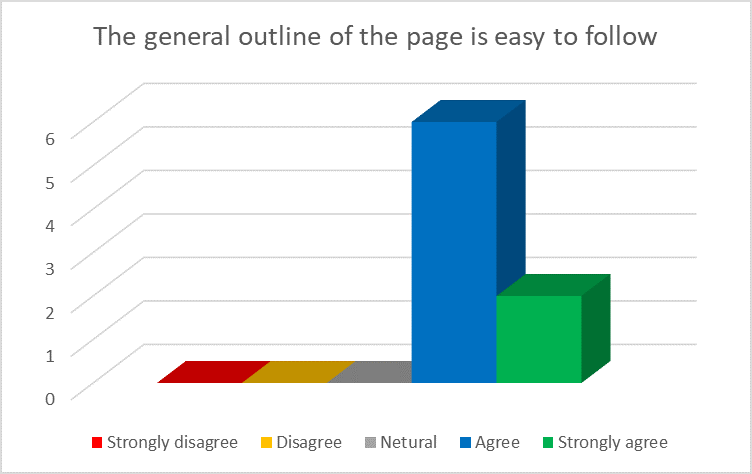
\includegraphics[width=0.8\linewidth]{Ex2/figures/q1} \end{center}

The ``Data Abstraction'' section gives a high-level look at what will be
analyzed.\\

\begin{center}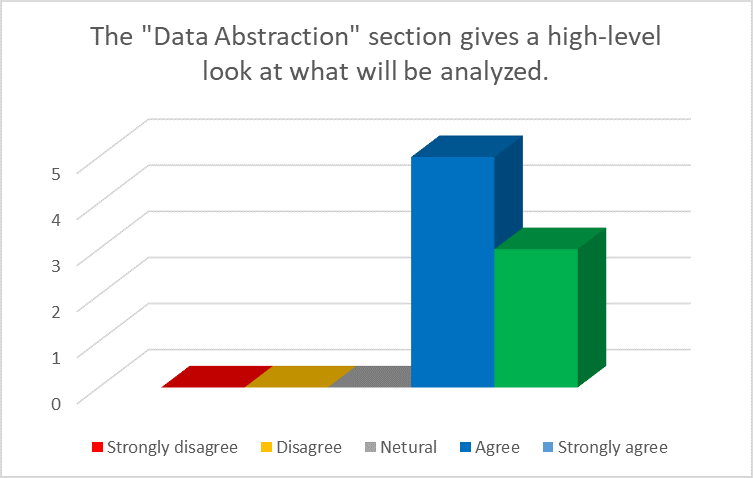
\includegraphics[width=0.8\linewidth]{Ex2/figures/q2} \end{center}

The ``Task Abstraction'' section is intuitive and easily understandable.

\begin{center}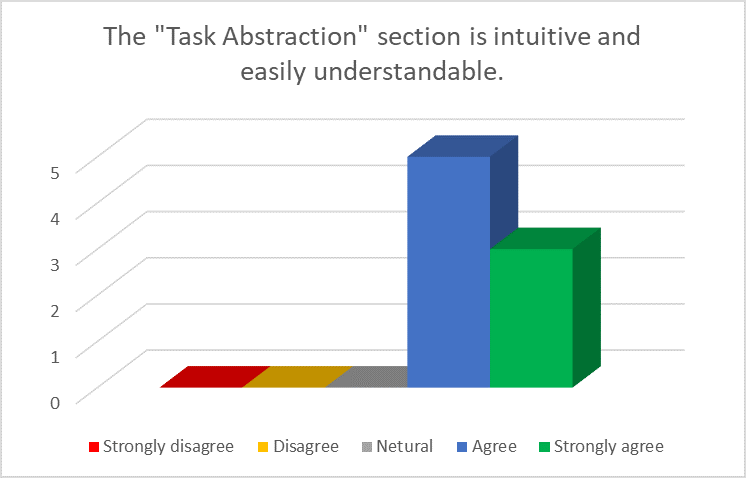
\includegraphics[width=0.8\linewidth]{Ex2/figures/q3} \end{center}

The ``Moving Average'' vizualization is easy to comprehend and
interpret.\\

\begin{center}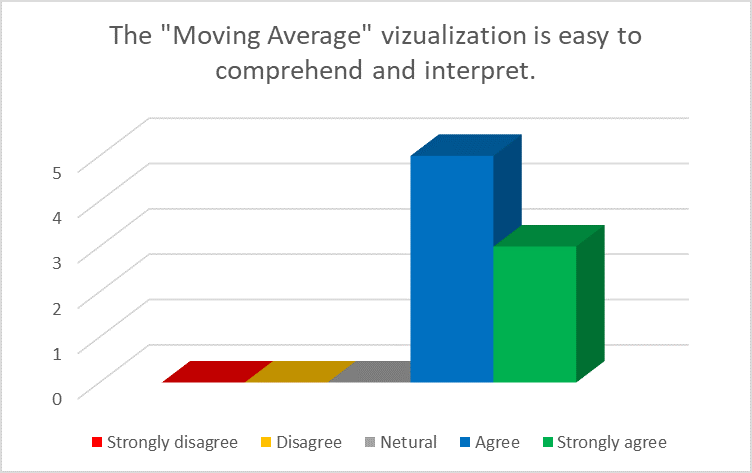
\includegraphics[width=0.8\linewidth]{Ex2/figures/q4} \end{center}

The Parallel Coordinate Plots (with and without box plots) helped
identify a trend.\\

\begin{center}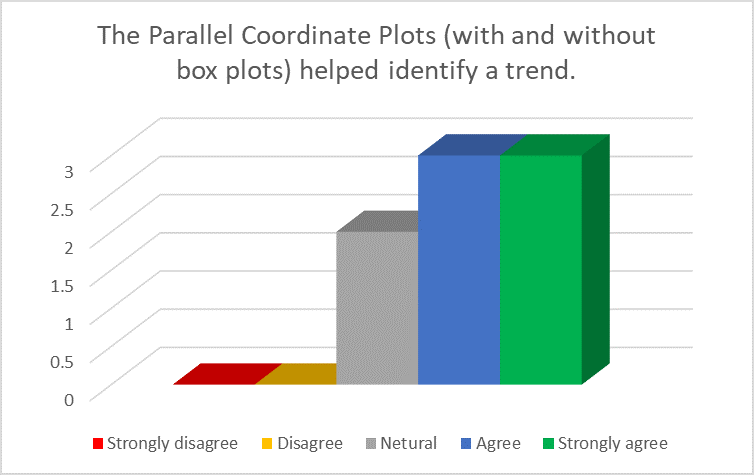
\includegraphics[width=0.8\linewidth]{Ex2/figures/q5} \end{center}

The heat map was helpful in identifying similarities between Months and
Years.

\begin{center}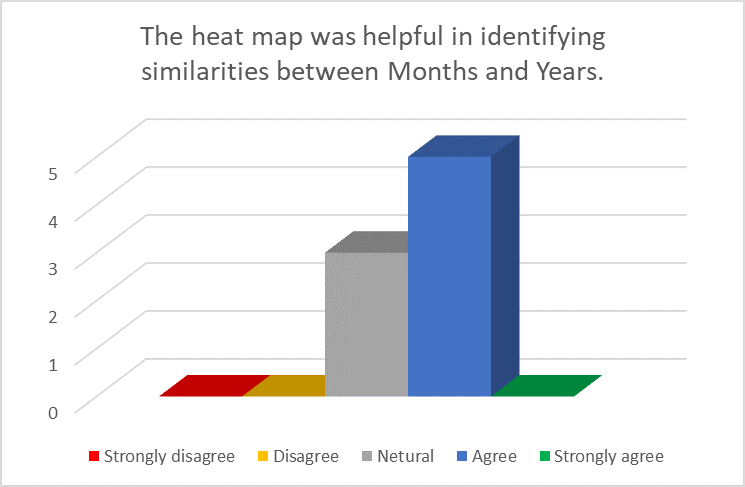
\includegraphics[width=0.8\linewidth]{Ex2/figures/q6} \end{center}

The stacked bar chart was helpful in comparing monthly trends for each
decade.\\

\begin{center}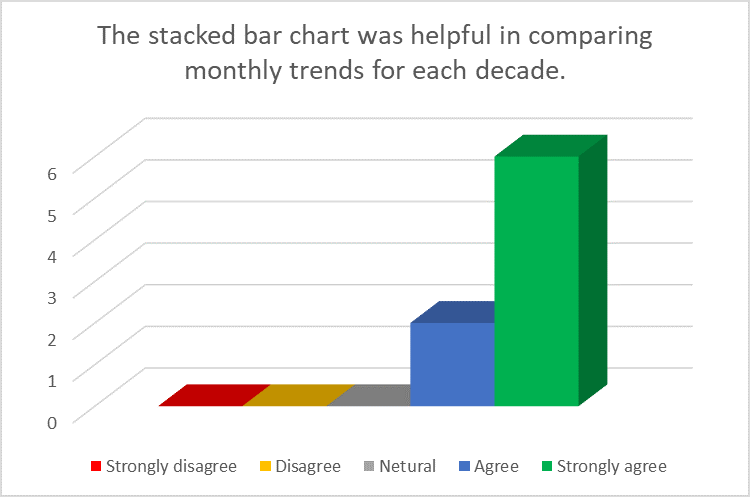
\includegraphics[width=0.8\linewidth]{Ex2/figures/q7} \end{center}

The stacked area chart was helpful in indentifying changes in snowfall
per month over time.

\begin{center}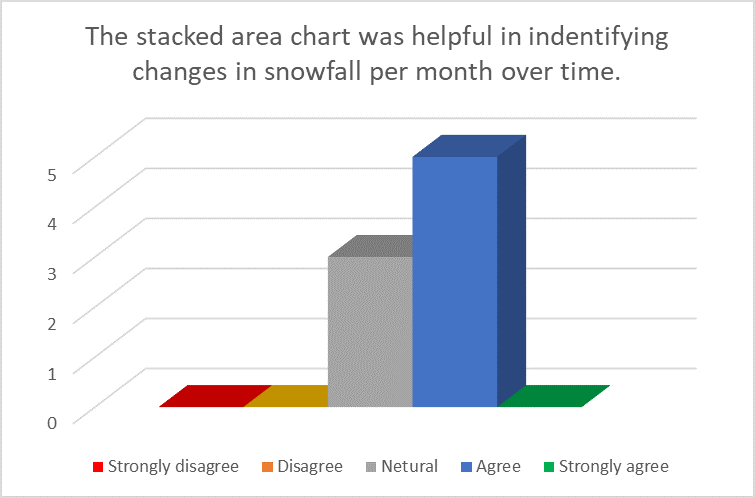
\includegraphics[width=0.8\linewidth]{Ex2/figures/q8} \end{center}

The side by side bar charts made it easy to compare 1910 snowfall per
month with 2010.

\begin{center}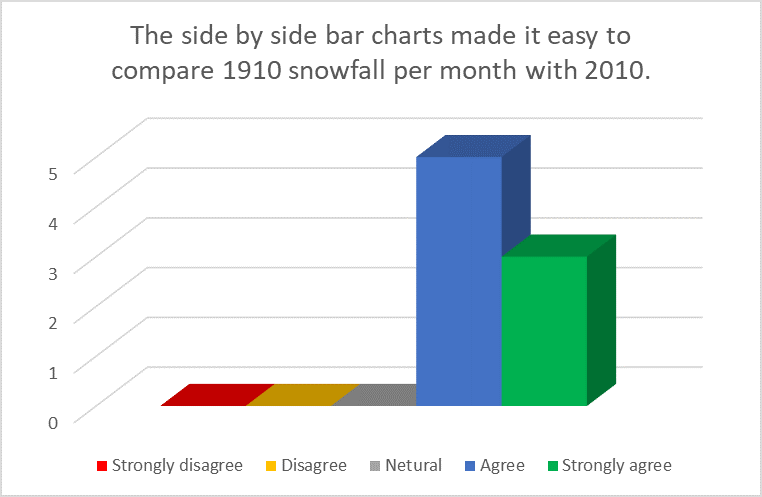
\includegraphics[width=0.8\linewidth]{Ex2/figures/q9} \end{center}

The 10 year forecast visualization matches expectation.\\

\begin{center}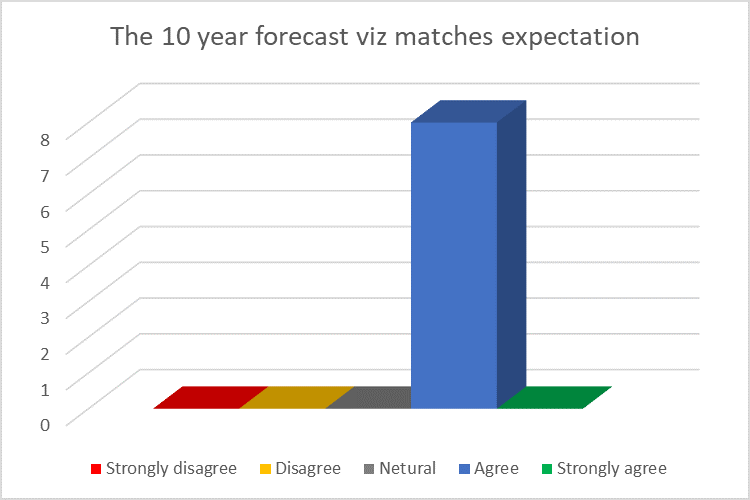
\includegraphics[width=0.8\linewidth]{Ex2/figures/q10} \end{center}

The forecast vizualization and explanation was easy to comprehend.\\

\begin{center}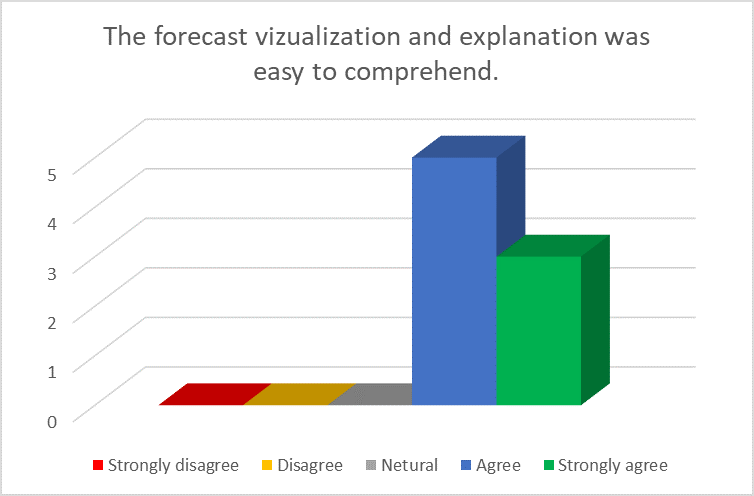
\includegraphics[width=0.8\linewidth]{Ex2/figures/q11} \end{center}

Each section answered the question that was asked.\\

\begin{center}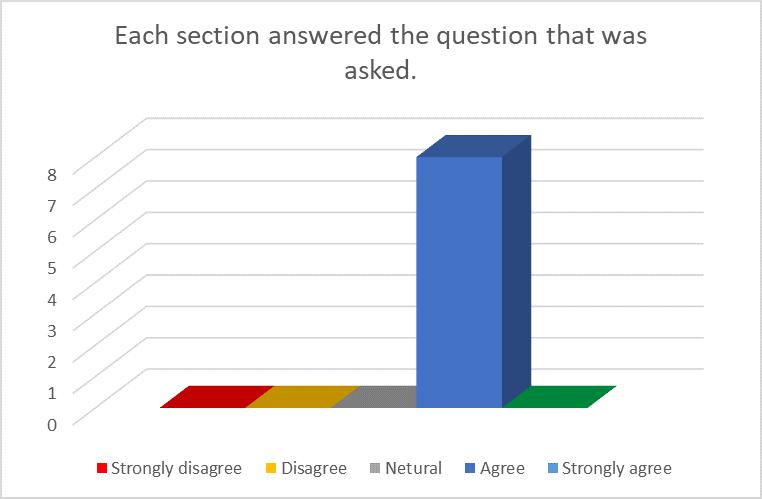
\includegraphics[width=0.8\linewidth]{Ex2/figures/q12} \end{center}

This analyses in this page all match my expectations of snowfall in
Houghton County.

\begin{center}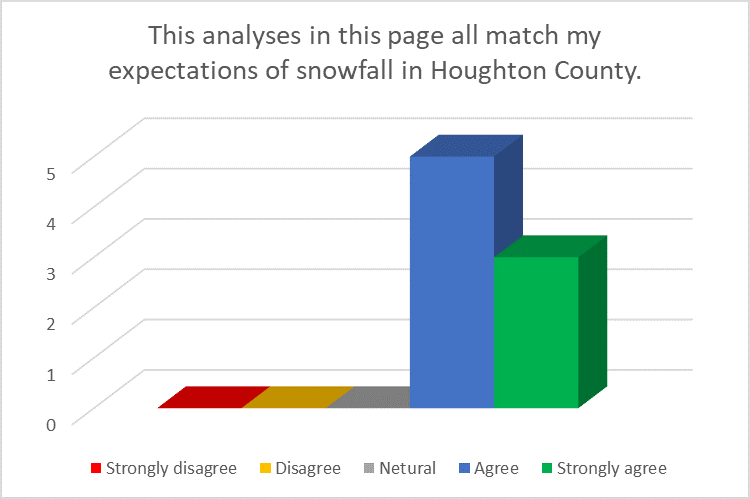
\includegraphics[width=0.8\linewidth]{Ex2/figures/q13} \end{center}


\end{document}
